\documentclass[11pt]{charter}
\usepackage[section]{placeins}
% El títulos de la memoria, se usa en la carátula y se puede usar el cualquier lugar del documento con el comando \ttitle
\titulo{Red de sensores WiFi para sistema productivo} 

% Nombre del posgrado, se usa en la carátula y se puede usar el cualquier lugar del documento con el comando \degreename
\posgrado{Carrera de Especialización en Sistemas Embebidos} 
%\posgrado{Carrera de Especialización en Internet de las Cosas} 
%\posgrado{Carrera de Especialización en Intelegencia Artificial}
%\posgrado{Maestría en Sistemas Embebidos} 
%\posgrado{Maestría en Internet de las cosas}

% Tu nombre, se puede usar el cualquier lugar del documento con el comando \authorname
\autor{Francisco G. Timez} 

% El nombre del director y co-director, se puede usar el cualquier lugar del documento con el comando \supname y \cosupname y \pertesupname y \pertecosupname
\director{Nombre del Director}
\pertenenciaDirector{pertenencia} 
% FIXME:NO IMPLEMENTADO EL CODIRECTOR ni su pertenencia
\codirector{} % si queda vacio no se deberíá incluir 
\pertenenciaCoDirector{}

% Nombre del cliente, quien va a aprobar los resultados del proyecto, se puede usar con el comando \clientename y \empclientename
\cliente{Pablo Scherf}
\empresaCliente{Cerámica FELI}

% Nombre y pertenencia de los jurados, se pueden usar el cualquier lugar del documento con el comando \jurunoname, \jurdosname y \jurtresname y \perteunoname, \pertedosname y \pertetresname.
\juradoUno{Nombre y Apellido (1)}
\pertenenciaJurUno{pertenencia (1)} 
\juradoDos{Nombre y Apellido (2)}
\pertenenciaJurDos{pertenencia (2)}
\juradoTres{Nombre y Apellido (3)}
\pertenenciaJurTres{pertenencia (3)}
 
\fechaINICIO{22 de junio de 2020}		%Fecha de inicio de la cursada de GdP \fechaInicioName
\fechaFINALPlanificacion{22 de Agosto de 2020} 	%Fecha de final de cursada de GdP
\fechaFINALTrabajo{22 de diciembre de 2020}		%Fecha de defensa pública del trabajo final


\begin{document}

\maketitle
\thispagestyle{empty}
\pagebreak


\thispagestyle{empty}
{\setlength{\parskip}{0pt}
\tableofcontents{}
}
\pagebreak


\section{Registros de cambios}
\label{sec:registro}


\begin{table}[ht]
\label{tab:registro}
\centering

\begin{tabularx}{\linewidth}{@{}|c|X|c|@{}}
\hline
\rowcolor[HTML]{C0C0C0} 
Revisión & \multicolumn{1}{c|}{\cellcolor[HTML]{C0C0C0}Detalles de los cambios realizados} & Fecha      \\ \hline
1.0      & Creación del documento                                                          & 22/06/2020 \\ \hline
1.1      & Avances hasta capítulo 6. Desglose de tareas									   & 10/07/2020 \\ \hline
1.2      & Se atendieron a las correcciones enviadas el día 14/07/2020                     & 15/07/2020 \\ \hline
\end{tabularx}
\end{table}

\pagebreak



\section{Acta de constitución del proyecto}
\label{sec:acta}

\begin{flushright}
Buenos Aires, \fechaInicioName
\end{flushright}

\vspace{2cm}

Por medio de la presente se acuerda con el Ing. \authorname\hspace{1px} que su Trabajo Final de la \degreename\hspace{1px} se titulará ``\ttitle'', consistirá esencialmente en el prototipo preliminar de un sensor de fácil configuración e instalación, para el registro de datos ambientales o de procesos específicos, y tendrá un presupuesto preliminar estimado en 640 hs y un costo estimado en xxxx pesos argentinos, con fecha de inicio \fechaInicioName\hspace{1px} y fecha de presentación pública \fechaFinalName.

Se adjunta a esta acta la planificación inicial.

\vfill

% Esta parte se construye sola con la información que hayan cargado en el preámbulo del documento y no debe modificarla
\begin{table}[ht]
\centering
\begin{tabular}{ccc}
\begin{tabular}[c]{@{}c@{}}Ariel Lutenberg \\ Director posgrado FIUBA\end{tabular} &  & \begin{tabular}[c]{@{}c@{}}\clientename \\ \empclientename \end{tabular} \vspace{2.5cm} \\ 
\multicolumn{3}{c}{\begin{tabular}[c]{@{}c@{}} \supname \\ Director del Trabajo Final\end{tabular}} \vspace{2.5cm} \\
\begin{tabular}[c]{@{}c@{}}\jurunoname \\ Jurado del Trabajo Final\end{tabular}     &  & \begin{tabular}[c]{@{}c@{}}\jurdosname\\ Jurado del Trabajo Final\end{tabular}  \vspace{2.5cm}  \\
\multicolumn{3}{c}{\begin{tabular}[c]{@{}c@{}} \jurtresname\\ Jurado del Trabajo Final\end{tabular}} \vspace{.5cm}                                                                     
\end{tabular}
\end{table}




\section{Descripción técnica-conceptual del proyecto a realizar}
\label{sec:descripcion}


En las PyMEs dedicadas a la industria ceramista, en la mayoría de las situaciones los emprendedores corrigen, a prueba y error, los parámetros de sus procesos productivos en base a los resultados obtenidos de la producción. Las correcciones se realizan según la experiencia propia del emprendedor y en la mayoría de los casos no se realizan registro de las variables del proceso.

Partiendo de la premisa que “lo que no se puede medir, no se puede mejorar”, se propone un sistema de fácil configuración e instalación, que les permita a estos emprendedores, en un principio, utilizar los criterios formados en la experiencia, y poder darles una base sólida en los datos para poder mejorar de manera continua.

Este proyecto debe ser de implementación sencilla, por dos motivos. Primero, no suelen tener un departamento dentro de la PyME dedicado al mantenimiento, pero si personal con conocimientos de electricidad industrial. Segundo, la estructura edilicia de la industria se modifica constantemente. Entonces debe ser un producto que se pueda reinstalar en otro sitio sin mayores inconvenientes.

Uno de los desafíos más importantes de este proyecto radica en reducir los costos de implementación, tiene que permitirle a la PyME instalar, desinstalar y reubicar los sensores con recursos propios, sin recurrir a mano de obra especializada.

El sistema consiste en nodos que se desarrollan en forma genérica y que pueden ser configurados según la necesidad de la PyME. Como se puede ver en la figura \ref{fig:diagBloques}, los nodos son similares, pero pueden tener distintas funciones asignadas, el Nodo 01 sensa temperatura y humedad, el Nodo 02 sensa temperatura y un switch (podría funcionar como contador) y el Nodo 03 tiene un módulo de expansión I2C. De esta manera, si algún Nodo pierde utilidad en el lugar donde se encuentra instalado, puede ser reubicado cambiando su configuración o no.


\vspace{10px}

\begin{figure}[htpb]
\centering 
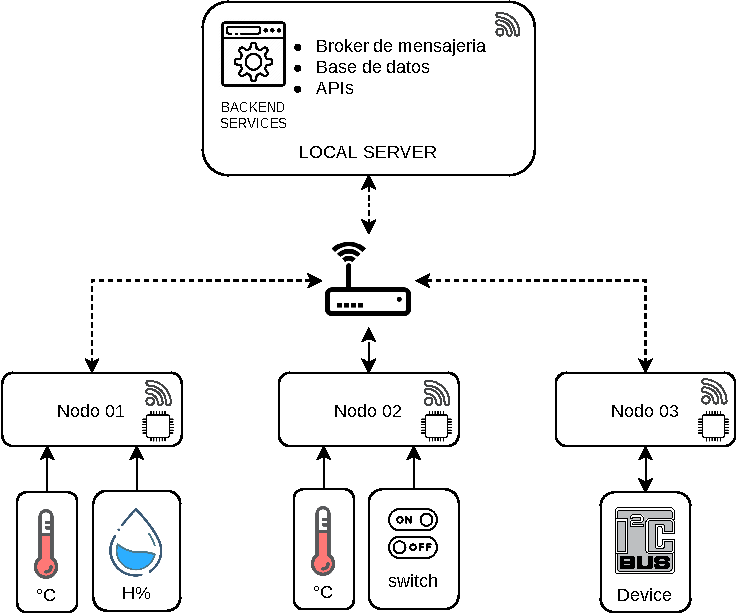
\includegraphics[width=.68\textwidth]{./Figuras/DiagramaEnBloques.pdf}
\caption{Diagrama en bloques del sistema}
\label{fig:diagBloques}
\end{figure}

\vspace{10px}


\section{Identificación y análisis de los interesados}
\label{sec:interesados}

\begin{table}[ht]
%\caption{Identificación de los interesados}
%\label{tab:interesados}
\begin{tabularx}{\linewidth}{@{}|l|X|X|l|@{}}
\hline
\rowcolor[HTML]{C0C0C0} 
Rol				& Nombre y Apellido & Organización 		& Puesto 	\\ \hline
Auspiciante		&					&					&			\\
Cliente			& \clientename      & \empclientename	& Gerente  	\\ 
Impulsor		&					&					&			\\	\hline
Responsable		& \authorname       & FIUBA        		& Alumno 	\\ \hline
Orientador		& \supname	      	& \pertesupname 	& Director	Trabajo final \\ \hline
Usuario final	& Personal técnico  & PyME           	& -       	\\ \hline
\end{tabularx}
\end{table}

\section{1. Propósito del proyecto}
\label{sec:proposito}

El propósito de este proyecto es brindarle a la PyME un recurso técnico económico para lograr implementar un sistema de seguimiento a su proceso o línea productiva; que le permita sensar variables de producción y tener los datos disponibles en gráficos actualizados en tiempo real.

\section{2. Alcance del proyecto}
\label{sec:alcance}

El desarrollo del presente proyecto incluye:
\begin{itemize}
\item Análisis, investigación y elección del hardware para el nodo.
\item Desarrollo de un prototipo de nodo que soporte distintos sensores detallados en los requerimientos.
\item Desarrollo del firmware del nodo.
\item Software \textit{backend} para almacenar los datos de los sensores en una base de datos tipo SQL.
\item Instalación de una interfaz gráfica estándar para visualización de los datos almacenados en la base de datos.
\end{itemize}

El proyecto NO incluye:
\begin{itemize}
\item Desarrollo de una interfaz web o gráfica específica para interactuar con los datos.
\item Desarrollo de una interfaz gráfica para configuración de los nodos.
\item Desarrollo de módulos de sensores para el nodo.
\item Pruebas de validación en campo.
\end{itemize}


\section{3. Supuestos del proyecto}
\label{sec:supuestos}

Para el desarrollo del presente proyecto se supone que:

\begin{itemize}
\item Los componentes electrónicos necesarios se consiguen dentro de territorio Argentino.
\item Se realizará un solo proceso de compra.
\item Los sensores son todos con salida digital, se supone que no requieren un proceso de calibración y ajuste.
\item La estructura de red WiFi existe y está en funcionamiento en la PyME.
\item La cobertura de la red WiFi es la adecuada para la línea productiva de la PyME.
\end{itemize}

\section{4. Requerimientos}
\label{sec:requerimientos}

Requerimientos del proyecto:

\begin{enumerate}
\item Requerimientos de hardware del nodo:
	\begin{enumerate}
	\item Debe soportar tensiones de alimentación de 5 Vdc a 24 Vdc.
	\item Debe basarse en el microcontrolador ESP8266 ó ESP32.
	\item Debe tener puerto de I2C para conectar otros módulos de expansión.
	\item Entradas:
		\begin{enumerate}
		\item Sensor de temperatura y humedad DHT22.
		\item Sensor de temperatura termopar K con MAX6675.
		\item Al menos una entrada para sensores con salida relé o transistorizados NPN.
		\end{enumerate}
	\end{enumerate}
\item Requerimientos de firmware del nodo:
	\begin{enumerate}
	\item Comunicación WiFi y por protocolo MQTT.
	\item Se debe poder configurar los sensores mediante un archivo JSON, con posibilidad de actualización mediante OTA.
	\item Se debe soportar actualización del firmware mediante OTA.
	\item Se debe soportar el módulo de expansión PCF8574.
	\end{enumerate}
\item Requerimientos de software backend:
	\begin{enumerate}
	\item Todos los servicios deben correr en una Raspberry Pi 3 o 4.
	\item Broker MQTT alojado en red local.
	\item Backend basado en Node-RED o NodeJS.
	\item Generación de tablas en base de datos SQL, según configuración del nodo.
	\item Dashboard web de variables sensadas mediante Grafana.
	\end{enumerate}
\end{enumerate}


\section{5. Entregables principales del proyecto}
\label{sec:entregables}

\begin{itemize}
\item Manual de configuración
\item Diagrama esquemático
\item Código fuente
\item Informe final
\end{itemize}

\section{6. Desglose del trabajo en tareas}
\label{sec:wbs}

\begin{enumerate}
\item Planificación del Proyecto (40 hs)
	\begin{enumerate}
	\item Elaboración del documento de planificación del proyecto (20 hs)
	\item Diseño de la arquitectura global del proyecto (20 hs)
	\end{enumerate}
\item Desarrollo del hardware del nodo (150 hs)
	\begin{enumerate}
	\item Diseño del diagrama esquemático (40 hs)
	\item Selección y compra de componentes (20 hs)
	\item Routeo PCB (40 hs)
	\item Fabricación del PCB (30 hs)
	\item Verificación y testing básico del prototipo (20 hs)
	\end{enumerate}
\item Desarrollo del firmware del nodo (210 hs)
	\begin{enumerate}
	\item Tests con freeRTOS (50 hs)
		\begin{enumerate}
		\item Generar tareas con los parámetros cargados desde un archivo JSON (25 hs)
		\item Actualización de tareas con la actualización del archivo JSON (25 hs)
		\end{enumerate}
	\item Diseño de la arquitectura de software (20 hs)
	\item Desarrollo de tareas para comunicación WiFi con broker de mensajería (20 hs)
	\item Desarrollo de las tareas para gestión de sensores (40 hs)
	\item Desarrollo de las tareas para gestión de puerto de expansión I2C (40 hs)
	\item Integración de todas las tareas desarrolladas (40 hs)
	\end{enumerate}
\item Desarrollo del backend (240 hs)
\begin{enumerate}
	\item Diseño de la arquitectura de software (40 hs)
	\item Instalación de broker de mensajería (40 hs)
	\item Desarrollo software de backend (100 hs)
		\begin{enumerate}
		\item Introducción a NodeJS (50 hs)
		\item Desarrollo bloque para comunicación con broker de mensajería (25 hs)
		\item Desarrollo bloque para inserción de datos en la base de datos (25 hs)
		\end{enumerate}
	\item Instalación y configuración de Grafana (20 hs)
	\item Integración de los bloques desarrollados (40 hs)
	\end{enumerate}
\end{enumerate}

Cantidad total de horas: (640 hs)

\section{7. Diagrama de Activity On Node}
\label{sec:AoN}

\begin{consigna}{red}
Armar el AoN a partir del WBS definido en la etapa anterior. 

%La figura \ref{fig:AoN} fue elaborada con el paquete latex tikz y pueden consultar la siguiente referencia \textit{online}:

%\url{https://www.overleaf.com/learn/latex/LaTeX_Graphics_using_TikZ:_A_Tutorial_for_Beginners_(Part_3)\%E2\%80\%94Creating_Flowcharts}

\end{consigna}

\begin{figure}[htpb]
\centering 
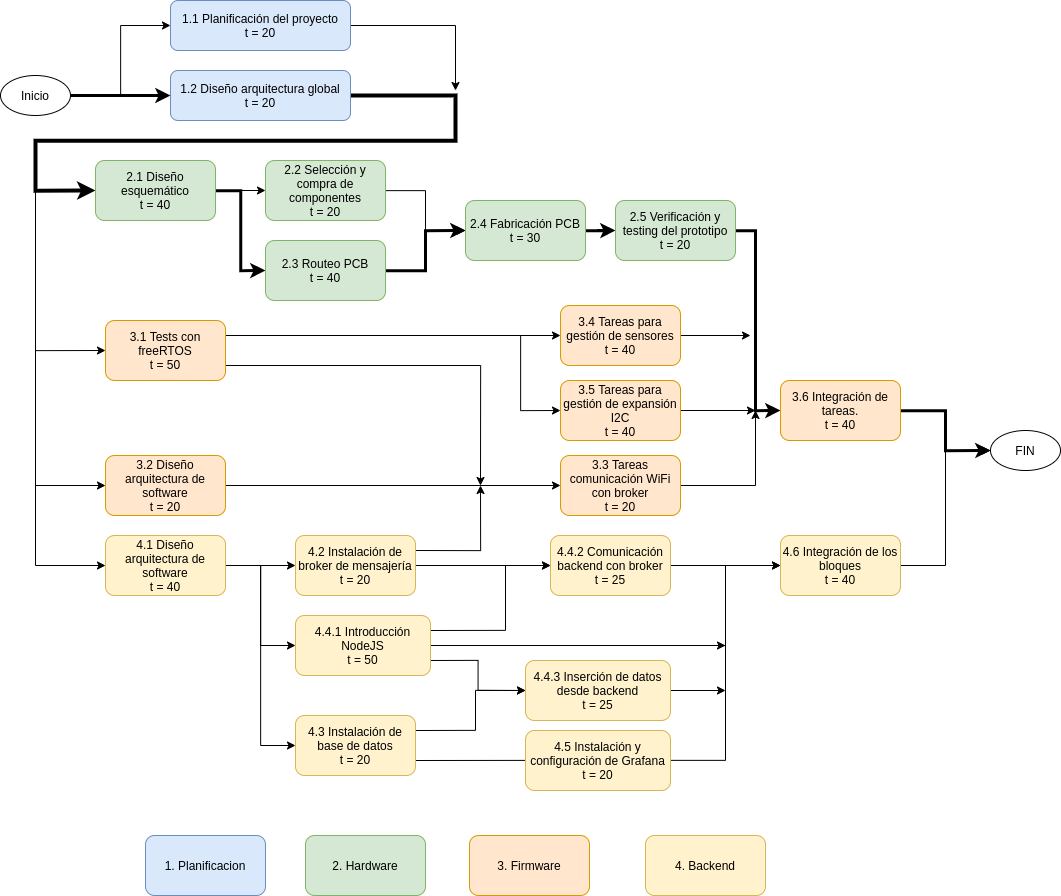
\includegraphics[width=.8\textwidth]{./Figuras/AoN.png}
\caption{Diagrama en \textit{Activity on Node}}
\label{fig:AoN}
\end{figure}

Indicar claramente en qué unidades están expresados los tiempos.
De ser necesario indicar los caminos semicríticos y analizar sus tiempos mediante un cuadro.
Es recomendable usar colores y un cuadro indicativo describiendo qué representa cada color, como se muestra en el siguiente ejemplo:



\section{8. Diagrama de Gantt}
\label{sec:gantt}

\begin{consigna}{red}
Utilizar el software Gantter for Google Drive o alguno similar para dibujar el diagrama de Gantt.

Existen muchos programas y recursos \textit{online} para hacer diagramas de gantt, entre las cuales destacamos:

\begin{itemize}
\item Planner
\item GanttProject
\item Trello + \textit{plugins}. En el siguiente link hay un tutorial oficial: \\ \url{https://blog.trello.com/es/diagrama-de-gantt-de-un-proyecto}
\item Creately, herramienta online colaborativa. \\\url{https://creately.com/diagram/example/ieb3p3ml/LaTeX}
\item Se puede hacer en latex con el paquete \textit{pgfgantt}\\ \url{http://ctan.dcc.uchile.cl/graphics/pgf/contrib/pgfgantt/pgfgantt.pdf}
\end{itemize}

Pegar acá una captura de pantalla del diagrama de Gantt, cuidando que la letra sea suficientemente grande como para ser legible. 
Si el diagrama queda demasiado ancho, se puede pegar primero la ``tabla'' del Gantt y luego pegar la parte del diagrama de barras del diagrama de Gantt.

Configurar el software para que en la parte de la tabla muestre los códigos del EDT (WBS).\\
Configurar el software para que al lado de cada barra muestre el nombre de cada tarea.\\
Revisar que la fecha de finalización coincida con lo indicado en el Acta Constitutiva.

En la figura \ref{fig:gantt}, se muestra un ejemplo de diagrama de gantt realizado con el paquete de \textit{pgfgantt}. En la plantilla pueden ver el código que lo genera y usarlo de base para construir el propio.

\begin{figure}[htbp]
\begin{center}
\begin{ganttchart}{1}{12}
  \gantttitle{2020}{12} \\
  \gantttitlelist{1,...,12}{1} \\
  \ganttgroup{Group 1}{1}{7} \\
  \ganttbar{Task 1}{1}{2} \\
  \ganttlinkedbar{Task 2}{3}{7} \ganttnewline
  \ganttmilestone{Milestone o hito}{7} \ganttnewline
  \ganttbar{Final Task}{8}{12}
  \ganttlink{elem2}{elem3}
  \ganttlink{elem3}{elem4}
\end{ganttchart}
\end{center}
\caption{Diagrama de gantt de ejemplo}
\label{fig:gantt}
\end{figure}

\end{consigna}

\section{9. Matriz de uso de recursos de materiales}
\label{sec:recursos}


\begin{table}[htpb]
\label{tab:recursos}
\centering
\begin{tabularx}{\linewidth}{@{}|c|X|X|X|X|X|@{}}
\hline
\cellcolor[HTML]{C0C0C0} & \cellcolor[HTML]{C0C0C0} & \multicolumn{4}{c|}{\cellcolor[HTML]{C0C0C0}Recursos requeridos (horas)} \\ \cline{3-6} 
\multirow{-2}{*}{\cellcolor[HTML]{C0C0C0}\begin{tabular}[c]{@{}c@{}}Código\\ WBS\end{tabular}} & \multirow{-2}{*}{\cellcolor[HTML]{C0C0C0}\begin{tabular}[c]{@{}c@{}}Nombre \\ tarea\end{tabular}} & Material 1 & Material 2 & Material 3 & Material 4 \\ \hline
 &  &  &  &  &  \\ \hline
 &  &  &  &  &  \\ \hline
 &  &  &  &  &  \\ \hline
 &  &  &  &  &  \\ \hline
\end{tabularx}%
\end{table}


\section{10. Presupuesto detallado del proyecto}
\label{sec:presupuesto}

\begin{consigna}{red}
Si el proyecto es complejo entonces separarlo en partes:
\begin{itemize}
\item Un total global, indicando el subtotal acumulado por cada una de las áreas.
\item El desglose detallado del subtotal de cada una de las áreas.
\end{itemize}

IMPORTANTE: No olvidarse de considerar los COSTOS INDIRECTOS.

\end{consigna}

\begin{table}[htpb]
\centering
\begin{tabularx}{\linewidth}{@{}|X|c|r|r|@{}}
\hline
\rowcolor[HTML]{C0C0C0} 
\multicolumn{4}{|c|}{\cellcolor[HTML]{C0C0C0}COSTOS DIRECTOS} \\ \hline
\rowcolor[HTML]{C0C0C0} 
Descripción &
  \multicolumn{1}{c|}{\cellcolor[HTML]{C0C0C0}Cantidad} &
  \multicolumn{1}{c|}{\cellcolor[HTML]{C0C0C0}Valor unitario} &
  \multicolumn{1}{c|}{\cellcolor[HTML]{C0C0C0}Valor total} \\ \hline
 &
  \multicolumn{1}{c|}{} &
  \multicolumn{1}{c|}{} &
  \multicolumn{1}{c|}{} \\ \hline
 &
  \multicolumn{1}{c|}{} &
  \multicolumn{1}{c|}{} &
  \multicolumn{1}{c|}{} \\ \hline
\multicolumn{1}{|l|}{} &
   &
   &
   \\ \hline
\multicolumn{1}{|l|}{} &
   &
   &
   \\ \hline
\multicolumn{3}{|c|}{SUBTOTAL} &
  \multicolumn{1}{c|}{} \\ \hline
\rowcolor[HTML]{C0C0C0} 
\multicolumn{4}{|c|}{\cellcolor[HTML]{C0C0C0}COSTOS INDIRECTOS} \\ \hline
\rowcolor[HTML]{C0C0C0} 
Descripción &
  \multicolumn{1}{c|}{\cellcolor[HTML]{C0C0C0}Cantidad} &
  \multicolumn{1}{c|}{\cellcolor[HTML]{C0C0C0}Valor unitario} &
  \multicolumn{1}{c|}{\cellcolor[HTML]{C0C0C0}Valor total} \\ \hline
\multicolumn{1}{|l|}{} &
   &
   &
   \\ \hline
\multicolumn{1}{|l|}{} &
   &
   &
   \\ \hline
\multicolumn{1}{|l|}{} &
   &
   &
   \\ \hline
\multicolumn{3}{|c|}{SUBTOTAL} &
  \multicolumn{1}{c|}{} \\ \hline
\rowcolor[HTML]{C0C0C0}
\multicolumn{3}{|c|}{TOTAL} &
   \\ \hline
\end{tabularx}%
\end{table}


\section{11. Matriz de asignación de responsabilidades}
\label{sec:responsabilidades}
\begin{consigna}{red}
Establecer la matriz de asignación de responsabilidades y el manejo de la autoridad completando la siguiente tabla:

\begin{table}[htpb]
\centering
\resizebox{\textwidth}{!}{%
\begin{tabular}{|c|c|c|c|c|c|}
\hline
\rowcolor[HTML]{C0C0C0} 
\cellcolor[HTML]{C0C0C0} &
  \cellcolor[HTML]{C0C0C0} &
  \multicolumn{4}{c|}{\cellcolor[HTML]{C0C0C0}Listar todos los nombres y roles del proyecto} \\ \cline{3-6} 
\rowcolor[HTML]{C0C0C0} 
\cellcolor[HTML]{C0C0C0} &
  \cellcolor[HTML]{C0C0C0} &
  Responsable &
  Orientador &
  Equipo &
  Cliente \\ \cline{3-6} 
\rowcolor[HTML]{C0C0C0} 
\multirow{-3}{*}{\cellcolor[HTML]{C0C0C0}\begin{tabular}[c]{@{}c@{}}Código\\ WBS\end{tabular}} &
  \multirow{-3}{*}{\cellcolor[HTML]{C0C0C0}Nombre de la tarea} &
  \authorname &
  \supname &
  Nombre de alguien &
  \clientename \\ \hline
 &  &  &  &  &  \\ \hline
 &  &  &  &  &  \\ \hline
 &  &  &  &  &  \\ \hline
\end{tabular}%
}
\end{table}

{\footnotesize
Referencias:
\begin{itemize}
	\item P = Responsabilidad Primaria
	\item S = Responsabilidad Secundaria
	\item A = Aprobación
	\item I = Informado
	\item C = Consultado
\end{itemize}
} %footnotesize

Una de las columnas debe ser para el Director, ya que se supone que participará en el proyecto.
A su vez se debe cuidar que no queden muchas tareas seguidas sin ``A'' o ``I''.

Importante: es redundante poner ``I/A'' o ``I/C'', porque para aprobarlo o responder consultas primero la persona debe ser informada.

\end{consigna}

\section{12. Gestión de riesgos}
\label{sec:riesgos}

\begin{consigna}{red}
a) Identificación de los riesgos (al menos cinco) y estimación de sus consecuencias:
 
Riesgo 1: detallar el riesgo (riesgo es algo que si ocurre altera los planes previstos)
\begin{itemize}
\item Severidad (S): mientras más severo, más alto es el número (usar números del 1 al 10).\\
Justificar el motivo por el cual se asigna determinado número de severidad (S).
\item Probabilidad de ocurrencia (O): mientras más probable, más alto es el número (usar del 1 al 10).\\
Justificar el motivo por el cual se asigna determinado número de (O). 
\end{itemize}   

Riesgo 2:
\begin{itemize}
\item Severidad (S): 
\item Ocurrencia (O):
\end{itemize}

Riesgo 3:
\begin{itemize}
\item Severidad (S): 
\item Ocurrencia (O):
\end{itemize}


b) Tabla de gestión de riesgos:      (El RPN se calcula como RPN=SxO)

\begin{table}[htpb]
\centering
\begin{tabularx}{\linewidth}{@{}|X|c|c|c|c|c|c|@{}}
\hline
\rowcolor[HTML]{C0C0C0} 
Riesgo & S & O & RPN & S* & O* & RPN* \\ \hline
       &   &   &     &    &    &      \\ \hline
       &   &   &     &    &    &      \\ \hline
       &   &   &     &    &    &      \\ \hline
       &   &   &     &    &    &      \\ \hline
       &   &   &     &    &    &      \\ \hline
\end{tabularx}%
\end{table}

Criterio adoptado: 
Se tomarán medidas de mitigación en los riesgos cuyos números de RPN sean mayores a ....

Nota: los valores marcados con (*) en la tabla corresponden luego de haber aplicado la mitigación.

c) Plan de mitigación de los riesgos que originalmente excedían el RPN máximo establecido:
 
Riesgo 1: Plan de mitigación (si por el RPN fuera necesario elaborar un plan de mitigación).
  Nueva asignación de S y O, con su respectiva justificación:
  - Severidad (S): mientras más severo, más alto es el número (usar números del 1 al 10).
          Justificar el motivo por el cual se asigna determinado número de severidad (S).
  - Probabilidad de ocurrencia (O): mientras más probable, más alto es el número (usar del 1 al 10).
          Justificar el motivo por el cual se asigna determinado número de (O).

Riesgo 2: Plan de mitigación (si por el RPN fuera necesario elaborar un plan de mitigación).
 
Riesgo 3: Plan de mitigación (si por el RPN fuera necesario elaborar un plan de mitigación)

\end{consigna}


\section{13. Gestión de la calidad}
\label{sec:calidad}

\begin{consigna}{red}
Para cada uno de los requerimientos del proyecto indique:
\begin{itemize} 
\item Req \#1: Copiar acá el requerimiento.

Verificación y validación:

\begin{itemize}
\item Verificación para confirmar si se cumplió con lo requerido antes de mostrar el sistema al cliente:\\
Detallar 
\item Validación con el cliente para confirmar que está de acuerdo en que se cumplió con lo requerido:\\
Detallar  
\end{itemize}

\end{itemize}

Tener en cuenta que en este contexto se pueden mencionar simulaciones, cálculos, revisión de hojas de datos, consulta con expertos, etc.

\end{consigna}

\section{14. Comunicación del proyecto}
\label{sec:comunicaciones}

\begin{consigna}{red}
El plan de comunicación del proyecto es el siguiente:
\end{consigna}

% Please add the following required packages to your document preamble:
% \usepackage{graphicx}
% \usepackage[table,xcdraw]{xcolor}
% If you use beamer only pass "xcolor=table" option, i.e. \documentclass[xcolor=table]{beamer}
\begin{table}[htpb]
\centering
\resizebox{\textwidth}{!}{%
\begin{tabular}{|c|c|c|c|c|c|}
\hline
\rowcolor[HTML]{C0C0C0} 
\multicolumn{6}{|c|}{\cellcolor[HTML]{C0C0C0}PLAN DE COMUNICACIÓN DEL PROYECTO}           \\ \hline
\rowcolor[HTML]{C0C0C0} 
¿Qué comunicar? & Audiencia & Propósito & Frecuencia & Método de comunicac. & Responsable \\ \hline
                &           &           &            &                      &             \\ \hline
                &           &           &            &                      &             \\ \hline
                &           &           &            &                      &             \\ \hline
                &           &           &            &                      &             \\ \hline
                &           &           &            &                      &             \\ \hline
\end{tabular}%
}
\end{table}

\section{15. Gestión de Compras}
\label{sec:compras}

\begin{consigna}{red}
En caso de tener que comprar elementos o contratar servicios:
a) Explique con qué criterios elegiría a un proveedor.
b) Redacte el Statement of Work correspondiente.
\end{consigna}

\section{16. Seguimiento y control}
\label{sec:seguimiento}

\begin{consigna}{red}
Para cada tarea del proyecto establecer la frecuencia y los indicadores con los se seguirá su avance y quién será el responsable de hacer dicho seguimiento y a quién debe comunicarse la situación (en concordancia con el Plan de Comunicación del proyecto).

El indicador de avance tiene que ser algo medible, mejor incluso si se puede medir en \% de avance. Por ejemplo,se pueden indicar en esta columna cosas como ``cantidad de conexiones ruteadeas'' o ``cantidad de funciones implementadas'', pero no algo genérico y ambiguo como ``\%'', porque el lector no sabe porcentaje de qué cosa.

\end{consigna}

\begin{table}[!htpb]
\centering
\begin{tabularx}{\linewidth}{@{}|X|X|X|X|X|X|@{}}
\hline
\rowcolor[HTML]{C0C0C0} 
\multicolumn{6}{|c|}{\cellcolor[HTML]{C0C0C0}SEGUIMIENTO DE AVANCE}                                                                       \\ \hline
\rowcolor[HTML]{C0C0C0} 
Tarea del WBS & Indicador de avance & Frecuencia de reporte & Resp. de seguimiento & Persona a ser informada & Método de comunic. \\ \hline
 &  &  &  &  &  \\ \hline
 &  &  &  &  &  \\ \hline
 &  &  &  &  &  \\ \hline
 &  &  &  &  &  \\ \hline
 &  &  &  &  &  \\ \hline
\end{tabularx}%
%}
\end{table}

\section{17. Procesos de cierre}    
\label{sec:cierre}

\begin{consigna}{red}
Establecer las pautas de trabajo para realizar una reunión final de evaluación del proyecto, tal que contemple las siguientes actividades:

\begin{itemize}
\item Pautas de trabajo que se seguirán para analizar si se respetó el Plan de Proyecto original:
 - Indicar quién se ocupará de hacer esto y cuál será el procedimiento a aplicar. 
\item Identificación de las técnicas y procedimientos útiles e inútiles que se utilizaron, y los problemas que surgieron y cómo se solucionaron:
 - Indicar quién se ocupará de hacer esto y cuál será el procedimiento para dejar registro.
\item Indicar quién organizará el acto de agradecimiento a todos los interesados, y en especial al equipo de trabajo y colaboradores:
  - Indicar esto y quién financiará los gastos correspondientes.
\end{itemize}

\end{consigna}


\end{document}
